
       
\section{Programação por Restrições}

\begin{frame}[fragile]
%[fragile, allowframebreaks=0.9]

    \frametitle{Programação por Restrições (PR) -- I}

   \begin{block}{}
     \begin{itemize}
     
      \item A Programação por Restrições (PR) é conhecida por \textit{Constraint Programming} ou simplesmente \textbf{CP}

      \pause
      \item Uma poderosa teoria (e técnica)  que  contorna a complexidade de certos problemas
      exponenciais
      
       
      \pause
      \item A PR encontrava-se inicialmente dentro da IA e PO, mas como várias outras, tornaram-se
      fortes e autônomas. Atualmente uma área de pesquisa bem forte em alguns países.
      
     
    \end{itemize}
    
    \end{block}
    
\end{frame}




\begin{frame}[fragile]
%[fragile, allowframebreaks=0.9]

    \frametitle{Programação por Restrições (PR) -- II}

   \begin{block}{}
     \begin{itemize}

      \item Aproximadamente o algoritmo da PR é dado:
       \pause       
          \begin{enumerate}

            \item Avaliar algebricamente  os domínios das variáveis com suas restrições

            \item Intercala iterativamente a \textsf{propagação de restrições} com 
                  um \textsf{algoritmo de busca}

            \item A cada variável instanciada, o processo é repetido sobre as demais variáveis, reduzindo progressivamente o espaço de busca

            \item Volte ao passo inicial até que os domínios permaneçam estáticos
            e que as variáveis apresentem instâncias consistentes
              
          \end{enumerate}
       
        \pause
       \item Este núcleo é uma busca por constantes otimizações

        \pause
       \item Uma das virtudes da PR: a legibilidade e clareza de suas soluções
       
    \end{itemize}
    
    \end{block}
    
\end{frame}


\begin{frame}[fragile]
%[fragile, allowframebreaks=0.9]
\frametitle{Programação por Restrições (PR) -- III}

   \begin{block}{}
     \begin{itemize}
    \item Problemas combinatoriais com domínio nos inteiros são bons candidatos a serem
       resolvidos por PR
       \pause
       \item Quando temos problemas que precisamos conhecer \textbf{todas} as respostas, 
    não apenas a melhor resposta
    
      \pause
      \item Quando necessitamos de respostas \textit{precisas} e não apenas as aproximadas.
       Há um custo  computacional a ser pago aqui!
        
        \pause
        \item



    \end{itemize}
    \end{block}
    
\end{frame}



\begin{frame}[fragile]
%[fragile, allowframebreaks=0.9]

\frametitle{Metodologia da  Construção de Modelos}

\begin{figure}[ht!]
\begin{center}

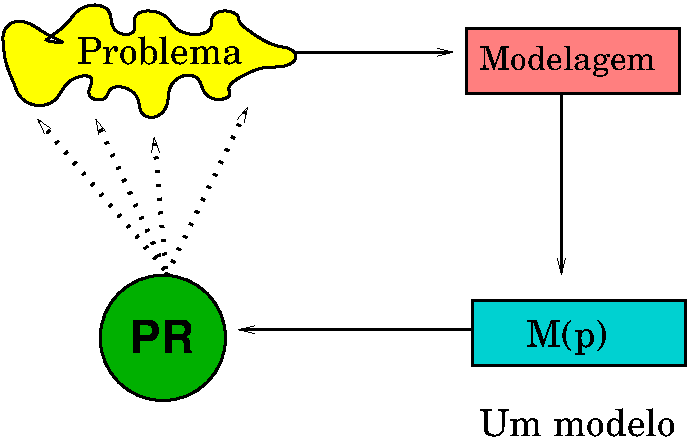
\includegraphics[width=0.70\textwidth, height=0.60\textheight]{figures/problema_modelagem.pdf}

\end{center}
\end{figure}


    
\end{frame}


\begin{frame}[fragile]
%[fragile, allowframebreaks=0.9]

\frametitle{Fluxo de Cálculo da PR}

\begin{figure}[!htb]
\centering
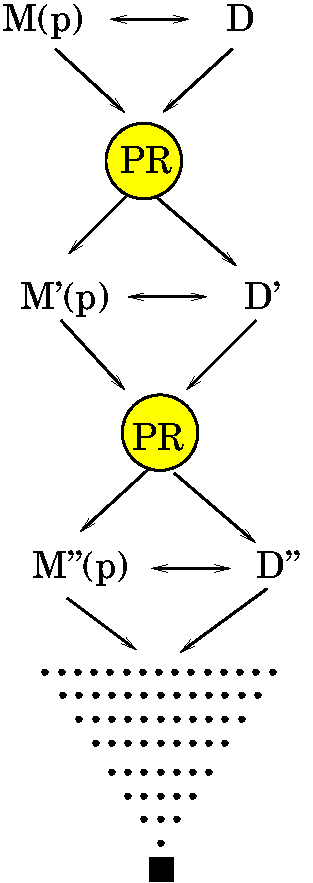
\includegraphics[width=0.30\textwidth, height=0.75\textheight]{figures/dinamica_pr.pdf}
\end{figure}
   
\end{frame}



\begin{frame}[fragile]
%[fragile, allowframebreaks=0.9]

\frametitle{Onde o objetivo da PR é:}

\begin{figure}[!htb]
\begin{center}
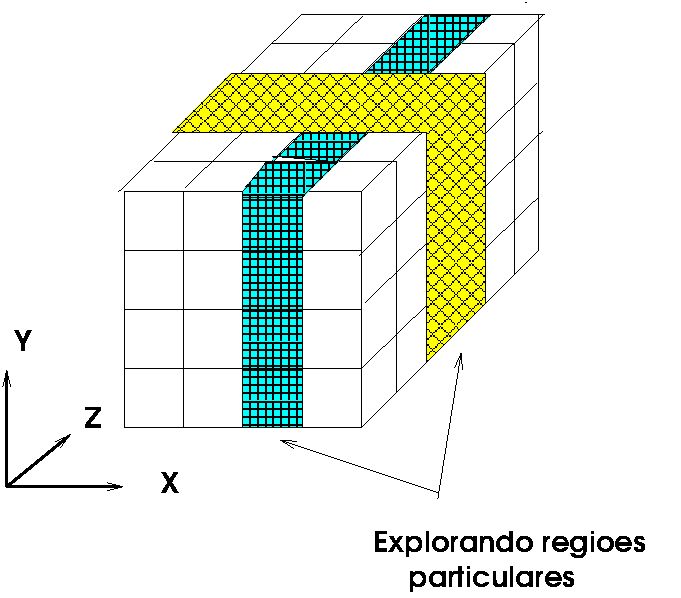
\includegraphics[width=0.70\textwidth, height=0.60\textheight]{figures/reducao_PR_01.pdf}
\caption{Realizar buscas com regiões reduzidas -- promissoras (regiões factíveis de soluções)}
\end{center}
\end{figure}
    
\end{frame}




\begin{frame}[fragile]
%[fragile, allowframebreaks=0.9]

\frametitle{Redução Iterativa em Sub-problemas}

\begin{figure}[!htb]

\begin{center}
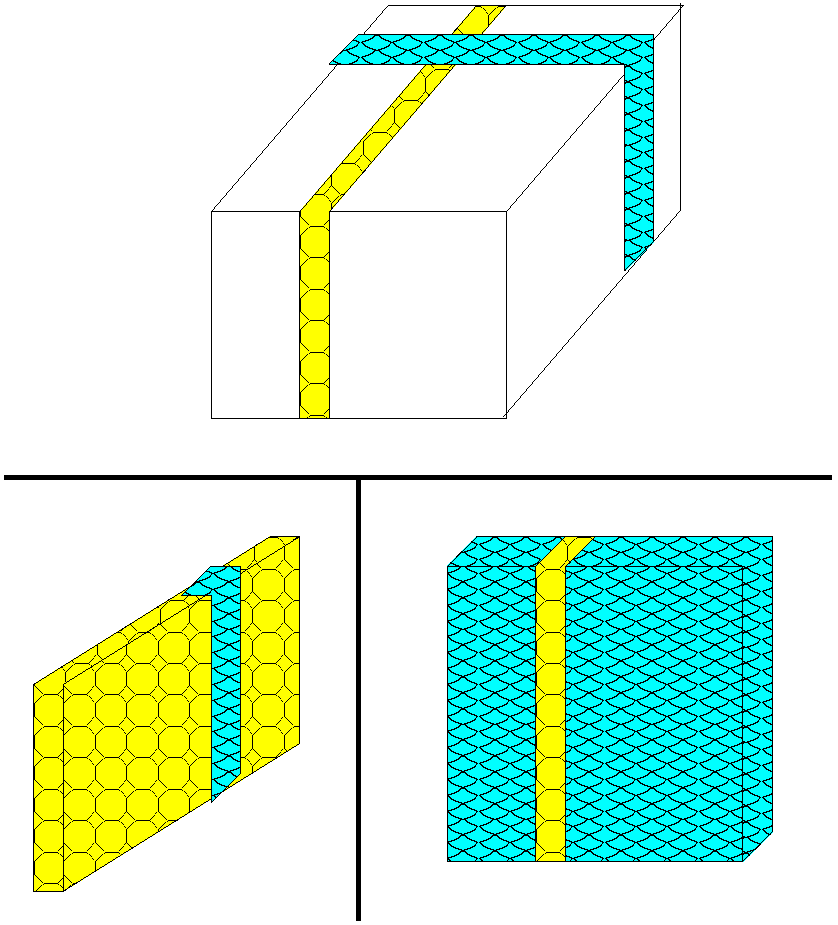
\includegraphics[width=0.70\textwidth, height=0.60\textheight]{figures/reducao_PR_02.pdf}
\caption{Redução de um CP em outros sub-problemas CPs equivalentes}
\end{center}
\end{figure}

    
\end{frame}


\begin{frame}[fragile] 

\frametitle{Exemplo -- 01 -- Soma de Números Primos}

\begin{itemize}
  \item Dado um número par qualquer, encontre  dois de números primos, $N_1$ e $N_2$,
diferentes entre si, que somados deêm este número 
par.

\pause
\item Exemplo:\\
Seja o PAR = 18\\
Uma soluç~ao:\\
$N_1 = 7$  e $N_2 = 11$\\
pois\\
$N_1 + N_2 = 18$
\end{itemize}

\end{frame}
%%%%%%%%%%%%%%%%%
\begin{frame}[fragile] 

\frametitle{Modelagem do Problema}

\begin{itemize}
  \item  $N_1$ e $N_2$ assumem valores no domínio dos números primos. \\
  Logo, é importante ter os números primos prontos!

  \pause
   \item A soma destes números é o par fornecido como entrada, $N_{PAR}$:\\
         $N_1 + N_2 = N_{PAR}$

  \pause
  \item  $N_1$ e $N_2$  são diferentes entre si\\
   $N_1 \neq N_2$

  \pause
  \item Como são inteiros: $N_1 < N_{PAR}$ e $N_2 < N_{PAR}$ \\
  Sim, é óbvio, mas isto faz uma redução significativa de domínio!

\end{itemize}

\end{frame}


%%%%%%%%%%%%%%%%%%%%%%%%%%
\begin{frame}[fragile]
 \frametitle{Código Completo}

\begin{itemize}
  \item Acompanhar as explicações do código de:\\
\url{https://github.com/claudiosa/CCS/blob/master/picat/soma_N1_N2_primos_CP.pi}

  \item Confira a execução e testes
\end{itemize}
\end{frame}


%%%%%%%%%%%%%%%%%%%%%%%%%%
\begin{frame}[fragile] 

\frametitle{Código em Partes}

\begin{small}
\begin{verbatim}
modelo => 
    PAR = 382,
    Variaveis = [N1,N2],
    % Gerando um domino soh de primos
    % L_dom = [I : I in 1..1000, eh_primo(I) == true],   %OU
    L_dom = [I : I in 1..1000, prime(I)],
    Variaveis :: L_dom,
\end{verbatim}
\end{small}
   
   Uma ótima estratégia: sair com um domínio de números candidatos!
    
\end{frame}
%%%%%%%%%%%%%%%%%
\begin{frame}[fragile] 

\frametitle{Código em Partes}

\begin{small}
\begin{verbatim}
    % RESTRICOES
    N1 #!= N2,
    N1 #< PAR,  
    N2 #< PAR,
    N1 + N2 #= PAR,
  
	% A BUSCA
	solve([ff], Variaveis),
  % UMA SAIDA
	printf("\n  N1: %d\t N2: %d", N1,N2),
	printf("\n.....................................")
	.
\end{verbatim}
\end{small}
    
\end{frame}
%%%%%%%%%%%%%%%%%
\begin{frame}[fragile] 

\frametitle{Código em Partes}

\begin{small}
\begin{verbatim}
import cp.

% main => modelo	.
% main ?=> modelo, fail.	
% main =>  true.	

main =>
    L = findall(_, $modelo),
    writef("\n Total de solucoes:  %d \n", length(L)) .

\end{verbatim}
\end{small}
    
\end{frame}


\begin{frame}[fragile]
%[fragile, allowframebreaks=0.9]

\frametitle{Saída -- I}

\begin{small}
\begin{verbatim}
Picat> cl('soma_N1_N2_primos_CP').
Compiling:: soma_N1_N2_primos_CP.pi
** Warning  : redefine_preimported_symbol(math): prime / 1
soma_N1_N2_primos_CP.pi compiled in 7 milliseconds
loading...

yes

Picat> main.                      

  N1: 3	 N2: 379
.....................................
  N1: 23	 N2: 359
.....................................
  N1: 29	 N2: 353
.....................................
\end{verbatim}
    
\end{small}
\end{frame}


\begin{frame}[fragile]
%[fragile, allowframebreaks=0.9]

\frametitle{Saída -- II}

\begin{small}
\begin{verbatim}
 .....................................
  N1: 353	 N2: 29
.....................................
  N1: 359	 N2: 23
.....................................
  N1: 379	 N2: 3
.....................................
 Total de solucoes:  18 

yes

Picat> 
\end{verbatim}
    
\end{small}
\end{frame}
%%%%%%%%%%%%%%%%%%%%%%%%%%%%%%%%%%%%%%%%%%%%%%%%%%%%%%%%%%%%%%%%%%%%
\begin{frame}[fragile] 

\frametitle{Exemplo -- 02 -- Escala de Consultórios}

\begin{itemize}
\item Seja um Posto Atendimento Médico, um PA, com 4 consultórios e 7 especialidades
  médicas

\pause
\item O problema é distribuir estes médicos nestes 4 consultórios
tal que alguns requisitos sejam atendidos (restrições  satisfeitas)

\pause
\item A abordagem aqui é ingênua e sem muitos critérios
\end{itemize}

\end{frame}
\begin{frame}[fragile] 

\frametitle{Modelagem do Problema}

\begin{itemize}
  \item  Vamos usar uma matriz bi-dimensional para 
  representar o problema. Linhas $\leftrightarrow$ consultórios (1 a 4), e 
  as colunas $\leftrightarrow$ dias da semana (1 a 5)

  \pause
  \item Esta matriz será preenchida com valores/códigos de 1 a 7, de acordo com a especialidade médica.
  
  \pause
  \item Assim o domínio da matriz \texttt{Quadro} ($4 \times 5$) será
  preenchida com um destes códigos.
   
  \pause
  \item Vamos utilizar restrições globais: \texttt{member} e \texttt{all\_different}

  \pause
  \item As restrições globais se aplicam sobre um conjunto de variáveis.


\end{itemize}

\end{frame}

%%%%%%%%%%%%%%%%%%%%%%%%%%%%%%%%%%%%%%%%%%%%%
\begin{frame}[fragile] 

\frametitle{Modelagem -- Comentários}

\begin{itemize}
  \item A fase de busca e propagação do comando 	\texttt{solve(Critérios, Variáveis)}, 
  há dezenas de combinações possíveis: consultar o guia do usuário
  
  \pause
  \item Tem-se os predicados extras ... são muitos, todos os da CP

  \pause
  \item Finalmente, exemplos sofisticados-- de PR com PICAT:\\
  \url{http://www.hakank.org/picat/} -- \textit{\textbf{My Picat page}} --
  por Hakan Kjellerstrand 

\end{itemize}

\end{frame}

%%%%%%%%%%%%%%%%%%%%%%%%%%
\begin{frame}[fragile]
 \frametitle{Código Completo}

\begin{itemize}
  \item Acompanhar as explicações do código de:\\
\url{https://github.com/claudiosa/CCS/blob/master/picat/horario_medico_CP.pi}

  \item Confira a execução e testes
\end{itemize}
\end{frame}


%%%%%%%%%%%%%%%%%%%%%%%%%%%%%%%%%%%%%%%%%%%%%%%%%%%%
\begin{frame}[fragile] 

\frametitle{Código em Partes}

\begin{small}
\begin{verbatim}
modelo => 
    Dias = 5, % segunda= 1, ...., sexta-feira = 5
    Consultorio = 4,
    L_dom = [ oftalmo, otorrino, pediatra,  gineco, 
%                1        2          3         4
              cardio, dermato, clin_geral ],
%                5       6        7
   Quadro = new_array(Consultorio, Dias ), %% Lin x Col
   Quadro :: 1 .. L_dom.len , %% operador len . "eh colado"
...
\end{verbatim}
\end{small}
   
    
\end{frame}
%%%%%%%%%%%%%%%%%%%%%%%%%%%%%%%%%%%%%%%%%%%%%%%%%%%%
\begin{frame}[fragile] 

\frametitle{Código em Partes}

\begin{small}
\begin{verbatim}
    %% O medico 2 NUNCA trabalha no consultorio 1
    foreach ( J in 1 .. Dias ) 
        Quadro[1,J] #!= 2
    end,
    
    %% O medico 5 NUNCA trabalha no consultorio 4
    foreach ( J in 1 .. Dias ) 
        Quadro[4,J] #!= 5
    end,
...
\end{verbatim}
\end{small}
    
\end{frame}
%%%%%%%%%%%%%%%%%%%%%%%%%%%%%%%%%%%%%%%%%%%%%%%%%%%%
\begin{frame}[fragile] 

\frametitle{Código em Partes}

\begin{small}
\begin{verbatim}

  %% O Clin Geral deve vir o maior numero de dias ... 
  %% Esta restricao eh matematicamente é HARD
   foreach ( I in 1 .. Consultorio )
     member(7,[Quadro[I,J] : J in 1..Dias]) 
   end,  
  
  %% Ninguém trabalha no mesmo consultorio em dias seguidos
  foreach ( J in 1 .. Dias )
      all_different( [Quadro[I,J] : I in 1..Consultorio] )
  end,  
 
  %% Ninguém trabalha no mesmo dia em mais de um consultorio
   foreach ( I in 1 .. Consultorio )
      all_different( [Quadro[I,J] : J in 1..Dias] )
   end,  
...  
\end{verbatim}
\end{small}
    
\end{frame}
%%%%%%%%%%%%%%%%%%%%%%%%%%%%%%%%%%%%%%%%%%%%%%%%%%%%
\begin{frame}[fragile] 

\frametitle{Código em Partes}

\begin{small}
\begin{verbatim}
	% A BUSCA
	solve([ff], Quadro),
  % UMA SAIDA
	
   printf("\n Uma escolha:"),
   print_matrix( Quadro ),
   print_matrix_NAMES( Quadro , L_dom ),
	 printf(".............................\n") .
\end{verbatim}
\end{small}
    
\end{frame}
%%%%%%%%%%%%%%%%%%%%%%%%%%%%%%%%%%%%%%%%%%%%%%%%%%%%
\begin{frame}[fragile] 

\frametitle{Código em Partes}

\begin{small}
\begin{verbatim}
print_matrix_NAMES( M, Lista ) =>
 L = M.length,
 C = M[1].length,
  nl,
   foreach(I in 1  .. L)
     foreach(J in 1  ..  C)
      printf(":%w \t" , print_n_lista( M[I,J], Lista) )
     % printf("(%d,%d): %w " , I, J, M[I,J] ) -- FINE
     end,
     nl
   end.
%%%%%%%%%%%%%%%%%%%%%%%%%%%%%%%%%%%%%%%%%%%%%%%%%%%%%%%%%%%%%%%%%%
print_n_lista( _, [] ) =  [].
print_n_lista( 1, [A|_] ) = A.
print_n_lista( N, [_|B] ) = print_n_lista( (N-1), B ) .
%%%%%%%%%%%%%%%%%%%%%%%%%%%%%%%%%%%%%%%%%%%%%%%%%%%%%%%%%%%%%%%%%%
\end{verbatim}
\end{small}
    
\end{frame}
%%%%%%%%%%%%%%%%%%%%%%%%%%%%%%%%%%%%%%%%%%%%%%%%%%%%


\begin{frame}[fragile]
%[fragile, allowframebreaks=0.9]

\frametitle{Saída - I}

\begin{small}
\begin{verbatim}
Picat> cl('horario_medico_CP.pi').
Compiling:: horario_medico_CP.pi
horario_medico_CP.pi compiled in 10 milliseconds
loading...

yes

Picat> main                       

 Uma escolha:
7 1 3 4 5 
4 7 2 3 1 
1 3 7 5 2 
3 2 1 7 4 
\end{verbatim}
  
\end{small}
\end{frame}

%%%%%%%%%%%%%%%%%%%%%%%%%%%%%%%%%%%%%%%%%%%%%%%%%%%%

\begin{frame}[fragile]
%[fragile, allowframebreaks=0.9]

\frametitle{Saída - II}

\begin{small}
\begin{verbatim}
:clin_geral 	:oftalmo 	:pediatra 	:gineco 	:cardio 	
:gineco 	:clin_geral 	:otorrino 	:pediatra 	:oftalmo 	
:oftalmo 	:pediatra 	:clin_geral 	:cardio 	:otorrino 	
:pediatra 	:otorrino 	:oftalmo 	:clin_geral 	:gineco 	
....................................
yes
\end{verbatim}
  
\end{small}
\end{frame}

\begin{frame}[fragile]
%[fragile, allowframebreaks=0.9]

\frametitle{Saída - III}

\begin{small}
\begin{verbatim}

$ time(picat horario_medico_CP.pi )

 Uma escolha:
7 1 3 4 5 
4 7 2 3 1 
1 3 7 5 2 
3 2 1 7 4 

:clin_geral 	:oftalmo 	:pediatra 	:gineco 	:cardio 	
:gineco 	:clin_geral 	:otorrino 	:pediatra 	:oftalmo 	
:oftalmo 	:pediatra 	:clin_geral 	:cardio 	:otorrino 	
:pediatra 	:otorrino 	:oftalmo 	:clin_geral 	:gineco 	
....................................
real	0m0,023s
user	0m0,007s
sys	0m0,013s
[ccs@gerzat picat]$ 
\end{verbatim}
  
\end{small}
\end{frame}

%%%%%%%%%%%%%%%%%%%%%%%%%%%%%%%%%%%%%%%%%%%%%%%%%%%%

\begin{frame}[fragile]
\frametitle{Reflexões}


\begin{itemize}
  \item Há outros métodos para se resolver estes problemas.\\
  Exemplo: Programação Linear, Buscas Heurísticas, etc

  \pause  
  \item As restrições globais se aplicam sobre um conjunto de variáveis
  e há muitas outras importantes disponíveis no Picat

  \pause
  \item A área é extensa, contudo, Picat adere há todos requisitos da PR

    \pause
  \item Resumo da PR: segue por uma notação/manipulação algébrica restrita,
        simplificar e bissecionar as restrições, instanciar variáveis, 
        verificar inconsistências,
        avançar sobre as demais variáveis, até que todas 
        estejam instanciadas.
  
\end{itemize}

\end{frame}
